    \documentclass{article}
    \usepackage{graphicx} % Required for inserting images
    \usepackage{indentfirst}
    \usepackage{amsmath}
    \usepackage{array}
    \usepackage{listings}
    \usepackage[utf8]{inputenc}
    \usepackage{float}
    \usepackage{minted}
    \title{Compte Rendu Projet}
    \author{Matéo Garcia, Aymeric Delehonte, Elliott Vanwormhoudt}
    \date{March 2023}

    \graphicspath{ {./images/} }

    \begin{document}

        \maketitle

    % PARTIE 1
        \section{Introduction}\label{sec:introduction}
        Durant cette semaine, nous avons tout d'abord réaliser une réunion avec notre enseignant référant pour voir et savoir comment débuter notre projet. A la suite de cette entrevue, nous avons eu une liste de tâches à réaliser qui sont les suivantes :
        \begin{itemize}
            \item Ecrire un modèle
            \item A la main, inventer une petite instance
            \item Ecrire le modèle de cette instance
            \item Ecrire le QUBO avec de nouvelles fonctions tel que add\_linear() ou add\_quadratic().
        \end{itemize}



    % PARTIE 2
        \section{Modélisation du modèle}\label{sec:modelisation-du-modele}


        Passons désormais à la réalisation du modèle quadratique.
        Soit X l'ensemble des villes.
        On note $|X|$ la cardinalité des villes.\\\\
        On définit :

        \begin{equation*}
            x_{ip} =
            \begin{cases}
                1 & \text{si on passe par la ville i a la p-eme position}\\
                0 & \text{sinon}
            \end{cases}
        \end{equation*}
        et $d_{ij}$ la distance entre les villes i et j.\\\\
        La fonction objectif du problème vise à obtenir la somme minimale des distances parcourues entre les villes. Cette somme est calculée en multipliant chaque ville i qui peut être visitée en position p par chaque ville j qui peut être visitée en position p+1, puis en multipliant le résultat par la distance entre la ville i et la ville j:

        \begin{equation*}
           \sum_{i=1}^{|X|}\sum_{\substack{j=1 \\ j\neq i }}^{|X|}(d_{ij}x_{i|X|}x_{j1}+ \sum_{p=1}^{|X|-1}d_{ij}x_{ip}x_{j(p+1))}\\
        \end{equation*}
        Cependant, la simple utilisation de cette équation ne suffit pas.
        En effet, il est possible que la solution actuelle traverse plusieurs fois une ville ou même qu'elle ne traverse pas toutes les villes. C'est pourquoi l'imposition de contraintes est nécessaire.

        Avant toute chose, il est important de garantir qu'il n'y ai qu'une seule ville par position. Pour cela, il faut s'assurer qu'une seule ville est choisie pour chaque position p. Cela signifie que la somme des variables binaires $x_{ip}$ doit être égale à 1 pour chaque p fixé.
        \begin{equation*}
            \begin{aligned}
                \forall p=1,\dots,|X| ,\sum_{i=1}^{|X|}x_{ip} = 1
            \end{aligned}
        \end{equation*}

        De même, pour chaque ville i, la somme des variables binaires $x_{ip}$ pour toutes les positions p doit être égale à 1. En d'autres termes, chaque ville ne peut être visitée qu'une seule fois et doit être assignée à une seule position :

        \begin{equation*}
            \begin{aligned}
                \forall i=1,\dots,|X| ,\sum_{p=1}^{|X|}x_{ip} = 1
            \end{aligned}
        \end{equation*}



    % PARTIE 3
        \section{Exemple d'instance}\label{sec:exemple-instance}

        Prenons un exemple avec 5 villes.Voici le tableau des distances:\\\\
        \begin{tabular}{|c|c|c|c|c|c|}
            \hline
            Villes & Lille & Paris & Metz & Lyon & Marseille \\
            \hline
            Lille & 0 & 225 & 393 & 728 & 983 \\
            \hline
            Paris & 225 & 0 & 330 & 466 & 775\\
            \hline
            Metz & 393 & 330 & 0 & 460 & 769 \\
            \hline
            Lyon & 728 & 466 & 460 & 0 & 301\\
            \hline
            Marseille & 983 & 775 & 769 & 301 & 0\\
            \hline
        \end{tabular}\\

        On obtient comme fonction : \\\\
        $f(X)=d_{12}*x_{11}x_{22}+d_{13}*x_{11}x_{32}+d_{14}*x_{11}x_{42}+d_{15}*x_{11}x_{52}+d_{21}*x_{21}x_{12}+d_{23}*x_{21}x_{32}+d_{24}*x_{21}x_{42}+d_{25}*x_{21}x_{52}+d_{31}*x_{31}x_{12}+d_{32}*x_{31}x_{22}+d_{34}*x_{31}x_{42}+d_{35}*x_{31}x_{52}+d_{41}*x_{41}x_{12}+d_{42}*x_{41}x_{22}+d_{43}*x_{41}x_{32}+d_{45}*x_{41}x_{52}+d_{51}*x_{51}x_{12}+d_{52}*x_{51}x_{22}+d_{53}*x_{51}x_{32}+d_{54}*x_{51}x_{42}+d_{12}*x_{12}x_{23}+d_{13}*x_{12}x_{33}+d_{14}*x_{12}x_{43}+d_{15}*x_{12}x_{53}+d_{21}*x_{22}x_{13}+d_{23}*x_{22}x_{33}+d_{24}*x_{22}x_{43}+d_{25}*x_{22}x_{53}+d_{31}*x_{32}x_{13}+d_{32}*x_{32}x_{23}+d_{34}*x_{32}x_{43}+d_{35}*x_{32}x_{53}+d_{41}*x_{42}x_{13}+d_{42}*x_{42}x_{23}+d_{43}*x_{42}x_{33}+d_{45}*x_{42}x_{53}+d_{51}*x_{52}x_{13}+d_{52}*x_{52}x_{23}+d_{53}*x_{52}x_{33}+d_{54}*x_{52}x_{43}+d_{12}*x_{13}x_{24}+d_{13}*x_{13}x_{34}+d_{14}*x_{13}x_{44}+d_{15}*x_{13}x_{54}+d_{21}*x_{23}x_{14}+d_{23}*x_{23}x_{34}+d_{24}*x_{23}x_{44}+d_{25}*x_{23}x_{54}+d_{31}*x_{33}x_{14}+d_{32}*x_{33}x_{24}+d_{34}*x_{33}x_{44}+d_{35}*x_{33}x_{54}+d_{41}*x_{43}x_{14}+d_{42}*x_{43}x_{24}+d_{43}*x_{43}x_{34}+d_{45}*x_{43}x_{54}+d_{51}*x_{53}x_{14}+d_{52}*x_{53}x_{24}+d_{53}*x_{53}x_{34}+d_{54}*x_{53}x_{44}+d_{12}*x_{14}x_{25}+d_{13}*x_{14}x_{35}+d_{14}*x_{14}x_{45}+d_{15}*x_{14}x_{55}+d_{21}*x_{24}x_{15}+d_{23}*x_{24}x_{35}+d_{24}*x_{24}x_{45}+d_{25}*x_{24}x_{55}+d_{31}*x_{34}x_{15}+d_{32}*x_{34}x_{25}+d_{34}*x_{34}x_{45}+d_{35}*x_{34}x_{55}+d_{41}*x_{44}x_{15}+d_{42}*x_{44}x_{25}+d_{43}*x_{44}x_{35}+d_{45}*x_{44}x_{55}+d_{51}*x_{54}x_{15}+d_{52}*x_{54}x_{25}+d_{53}*x_{54}x_{35}+d_{54}*x_{54}x_{45}+d_{12}*x_{15}x_{20}+d_{13}*x_{15}x_{30}+d_{14}*x_{15}x_{40}+d_{15}*x_{15}x_{50}+d_{21}*x_{25}x_{10}+d_{23}*x_{25}x_{30}+d_{24}*x_{25}x_{40}+d_{25}*x_{25}x_{50}+d_{31}*x_{35}x_{10}+d_{32}*x_{35}x_{20}+d_{34}*x_{35}x_{40}+d_{35}*x_{35}x_{50}+d_{41}*x_{45}x_{10}+d_{42}*x_{45}x_{20}+d_{43}*x_{45}x_{30}+d_{45}*x_{45}x_{50}+d_{51}*x_{55}x_{10}+d_{52}*x_{55}x_{20}+d_{53}*x_{55}x_{30}+d_{54}*x_{55}x_{40} \\$ \\

        Concernant les contraintes, nous en obtenons 10, 5 pour s'assurer qu'on passe au moins une fois par ville, et 5 pour s'assurer que chaque ville n'est présente qu'une fois
        \begin{equation*}
            \begin{aligned}
                C_{p_{1}} : x_{11}+x_{21}+x_{31}+x_{41}+x_{51} = 1\\
                C_{p_{2}} : x_{12}+x_{22}+x_{32}+x_{42}+x_{52} = 1\\
                C_{p_{3}} : x_{13}+x_{23}+x_{33}+x_{43}+x_{53} = 1\\
                C_{p_{4}} : x_{14}+x_{24}+x_{34}+x_{44}+x_{54} = 1\\
                C_{p_{5}} : x_{15}+x_{25}+x_{35}+x_{45}+x_{55} = 1\\
            \end{aligned}
        \end{equation*}
        \\
        \begin{equation*}
            \begin{aligned}
                C_{i_{1}} : x_{11}+x_{12}+x_{13}+x_{14}+x_{15} = 1\\
                C_{i_{2}} : x_{21}+x_{22}+x_{23}+x_{24}+x_{25} = 1\\
                C_{i_{3}} : x_{31}+x_{32}+x_{33}+x_{34}+x_{35} = 1\\
                C_{i_{4}} : x_{41}+x_{42}+x_{43}+x_{44}+x_{45} = 1\\
                C_{i_{5}} : x_{51}+x_{52}+x_{53}+x_{54}+x_{55} = 1\\
            \end{aligned}
        \end{equation*}
        \\
        On obtient alors comme solution optimal :
        S = [1,2,4,5,3] avec une distance total de 2154.



    % PARTIE 4
        \section{Passage au QUBO}\label{sec:passage-au-qubo}

        Pour passer du modèle quadratique que nous possédons, il faut relaxer les contraintes.\\\\

        \underline {Pourquoi doit-on relaxer les contraintes ?}\\\\
        Les contraintes du  modèle quadratique servent à décrire les conditions qui doivent être respectées pour que la solution d'un problème soit valide. Par exemple, dans notre cas du voyageur de commerce, une des contraintes principale est que toutes les villes doivent être visitées une fois.\\\\
        Cependant avec la machine D-Wave, l'algorithme d'annealing quantique n'est pas adapté pour traiter les problèmes d'optimisation contraints qui nécessitent la satisfaction de conditions supplémentaires pour trouver une solution. Cela est dû à la difficulté d'incorporer des contraintes dans la représentation du problème et le processus d'annealing.\\\\
        De plus, l'ajout de contraintes à un problème d'optimisation peut rapidement devenir inextricable même pour les ordinateurs classiques, car cela peut entraîner une augmentation exponentielle du Nbr. de variables nécessaires pour représenter le problème. Par conséquent, les machines de D-Wave ne sont généralement pas utilisées pour résoudre les problèmes d'optimisation contraints.\\\\

        Pour relaxer les contraintes, il faut les incorporer dans la fonction objective. Le but étant de minimiser celle ci, il faut donc pénaliser le résultat lorsque la solution de respecte pas les contraintes.Pour cela, on peut prendre comme valeurs :

        \begin{equation*}
            \begin{aligned}
                \forall p=1,\dots,|X|, \lambda(\sum_{i=1}^{|X|}x_{ip}-1)^{2}\\
                \forall i=1,\dots,|X| , \lambda(\sum_{p=1}^{|X|}x_{ip}-1)^{2}
            \end{aligned}
        \end{equation*}
        Ces deux valeurs vont donc pénaliser la fonction objective d'au moins $\lambda$\\\\
        Si la somme de toutes les variables $x_{ip}$ pour p allant de 1 à $|X|$ n'est pas égale à 1, cela signifie qu'il y a soit 0, soit 2 (ou plus) villes situées à la même position p. Dans ce cas, la valeur de la fonction objective augmentera car la valeur de lambda multipliée par la différence entre la somme et 1, au carré, ne sera pas égale à 0. Cette augmentation de la valeur de la fonction objective va à l'encontre de l'objectif d'optimisation.	\\\\
        Le facteur lambda est utilisé pour ajuster l'impact de la fonction objectif. Cependant, il est important de choisir la bonne valeur de lambda pour obtenir des solutions optimales tout en respectant les contraintes. Par exemple, une valeur élevée de lambda garantit le respect des contraintes, mais peut rendre difficile l'obtention de solutions avec des valeurs de chemin satisfaisantes. En revanche, une valeur faible de lambda peut conduire à des solutions de faible distance,mais augmenter le risque d'obtenir des solutions impossibles.\\
        On obtient alors comme QUBO :
        \begin{equation*}
            \sum_{i=1}^{|X|}\sum_{\substack{j=1 \\ j\neq i }}^{|X|}(d_{ij}x_{i|X|}x_{j1}+\sum_{p=1}^{|X|-1}d_{ij}x_{ip}x_{j(p+1))}\\ +\sum_{p=1}^{|X|}\lambda(\sum_{i=1}^{|X|}x_{ip} -1)^{2}+ \sum_{i=1}^{|X|}\lambda(\sum_{p=1}^{|X|}x_{ip} -1)^{2}
        \end{equation*}

        \section{Implémentation et tests}\label{sec:implementation-et-tests}

        \subsection{Génération d'instances}\label{subsec:generation-d'instances}
        Pour faire des tests, nous avons généré des instances de problèmes de voyageur de commerce.\\
        Pour cela, nous avons utilisé le format TSPLIB.\\
        Ce format est un format de fichier standard pour les problèmes de voyageur de commerce.\footnote{https://en.wikipedia.org/wiki/TSPLIB}\\\\
        \begin{lstlisting}[label={lst:tsplib}]
            NAME: data/tsp_10.tsp
            TYPE: TSP
            COMMENT:by Elliott vanwormhoudt
            DIMENSION: 10
            EDGE_WEIGH_TYPE: "EXPLICIT"
            EDGE_WEIGHT_FORMAT: "FULL_MATRIX"


            EDGE_WEIGHT_SECTION
            0  76  12  34  54  37  30  53  45  38
            76   0  85  84  82  71  92  43  58  61
            12  85   0  43  49  48  20  66  57  50
            34  84  43   0  87  15  63  46  30  24
            54  82  49  87   0  87  33  88  88  84
            37  71  48  15  87   0  67  31  15   9
            30  92  20  63  33  67   0  80  74  68
            53  43  66  46  88  31  80   0  16  22
            45  58  57  30  88  15  74  16   0   7
            38  61  50  24  84   9  68  22   7   0
            EOF
        \end{lstlisting}


        \subsection{Experimentations}\label{subsec:experimentations}

        Grâce à cette équation, il est désormais possible d'implémenter le modèle en python en utilisant l'API de dwave.\\
        Pour cela, nous avons utilisé le code suivant :
        \begin{minted}{python}
    def create_bqm_TSP(matrix):
        """Create a BQM for the TSP problem.
        Args:
            list[list]: A matrix of distances between cities.
        Returns:
            BinaryQuadraticModel: The bqm.
        """
        # create the binary quadratic model
        bqm = BinaryQuadraticModel.empty(dimod.BINARY)
        n = len(matrix)

        # add the quadratic terms for the distance between cities
        for i in range(n):
            for j in range(n):
                if i == j:
                    continue
                for p in range(n):
                    bqm.add_quadratic('x_{}_{}'.format(i, p), 'x_{}_{}'.format(j, (p+1)%n), matrix[i, j])


        # add the constraint that there is only one city visited at each position
        for i in range(n):
            for p in range(n):
                for q in range(p+1, n):
                    bqm.add_quadratic('x_{}_{}'.format(i, p), 'x_{}_{}'.format(i, q), 2*LAMBDA)
                bqm.add_linear('x_{}_{}'.format(i, p), -LAMBDA)
            bqm.offset += LAMBDA

        # add the constraint that each city is visited exactly once
        for p in range(n):
            for i in range(n):
                for j in range(i+1, n):
                    bqm.add_quadratic('x_{}_{}'.format(i, p), 'x_{}_{}'.format(j, p), 2*LAMBDA)
                bqm.add_linear('x_{}_{}'.format(i, p), -LAMBDA)
            bqm.offset += LAMBDA

        return bqm


        \end{minted}
        Ce code permet donc d'ajouter les différents liaisons quadratiques, mais aussi de rajouter les contraintes relaxées.\\
        Dans un premier temps, nous créons le BQM vide.
        Puis, nous ajoutons les liaisons quadratiques en utilisant la fonction add\_quadratic.\\
        Ensuite, nous ajoutons les contraintes relaxées en ajoutant à l'offset .\\
        Pour les contraintes, il a fallut remplacer le carré par des sommes. Pour cela, on a :

        \begin{equation*}
            \begin{aligned}
            (\sum_{i=1}^{|X|}x_{ip} -1)^{2} \\ (\sum_{i=1}^{|X|}x_{ip} -1) *(\sum_{i=1}^{|X|}x_{ip} -1)\\
            (\sum_{i=1}^{|X|}x_{ip})^2 - 2 \sum_{i=1}^{|X|}x_{ip} +1\\
            \text{or  } (\sum_{i=1}^{|X|}x_{ip})^2 = \sum_{i=1}^{|X|}x_{ip}^2 + 2 \sum_{i=1}^{|X|}\sum_{j>i}^{|X|}x_{ip}x_{jp}\\
            \end{aligned}
        \end{equation*}
        et comme $x_{ip}$ vaut 0 ou 1, alors $x_{ip}^{2}=x_{ip}$ ie :\\
        \begin{equation*}
            \begin{aligned}
            (\sum_{i=1}^{|X|}x_{ip})^2 = \sum_{i=1}^{|X|}x_{ip} + 2 \sum_{i=1}^{|X|}\sum_{j>i}^{|X|}x_{ip}x_{jp}
            \end{aligned}
        \end{equation*}
        Ce qui nous donne :
        \begin{equation*}
        (\sum_{i=1}^{|X|}x_{ip} -1)^{2} = \sum_{i=1}^{|X|}x_{ip} + 2 \sum_{i=1}^{|X|}\sum_{j>i}^{|X|}x_{ip}x_{jp}\\ - 2 \sum_{i=1}^{|X|}x_{ip} +1\\
        \end{equation*}
        En simplifiant, on obtient finalement:
        \begin{equation*}
        (\sum_{i=1}^{|X|}x_{ip} -1)^{2} =  2 \sum_{i=1}^{|X|}\sum_{j>i}^{|X|}x_{ip}x_{jp}\\ -  \sum_{i=1}^{|X|}x_{ip} +1\\
        \end{equation*}



        \subsection{Résultats}\label{subsec:resultats}
        Une fois le code implémenté, nous avons pu lancer les différents tests.\\
        Pour cela, nous nous sommes interessés à faire varier les paramètres suivants :
        \begin{itemize}
            \item Lambda
            \item Annealing time
            \item Topologies
        \end{itemize}



        \noindent{\underline{Annealing Time :}}\\
        Nous avons analysé la valeur de l'average energy pour une instance de 10 villes avec un annealing time qui variait de 0.5 à 2000.
        \begin{table}[h]
            \centering
            \begin{tabular}{|c|c|c|c|}
                \hline
                \textbf{Annealing time} & \textbf{Average energy} & \textbf{Num reads} & \textbf{Nbr. de Solutions}\\
                \hline
                0.5  & 6797 & 1000 & 0\\
                \hline
                1  & 6163 & 1000 & 0\\
                \hline
                10  & 2275 & 1000 & 1\\
                \hline
                100  & 1798 & 1000 & 3\\
                \hline
                1000  & 2063 & 750 & 0\\
                \hline
                2000 /2000 & 2051 & 375 & 0\\
                \hline
            \end{tabular}
            \caption{Résultats de l'average energy selon l'annealing time}
            \label{tab:annealing_time}
        \end{table}\\
        On constate que plus l'annealing time augmente, plus l'average energy diminue. On constate aussi que la valeur de num reads doit être diminuée si nous voulons pouvoir obtenir un résultat à partir de 1000 annealing time. \\\\
        \underline{Lambda :} \\
        Toujours dans le cas d'une instance de 10 villes, nous allons à présent annalyser la valeur de l'average time avec un lambda qui varie de 10 à 1000. \\
        \begin{table}[H]
            \centering
            \begin{tabular}{|c|c|c|}
                \hline
                \textbf{Lambda} & \textbf{Average energy} & \textbf{Nbr. de Solutions} \\
                \hline
                10  & 285 & 0\\
                \hline
                50  & 975 & 3\\
                \hline
                100  & 1857 & 1\\
                \hline
                200  & 3262 & 1\\
                \hline
                500  & 6160 & 2\\
                \hline
                1000  & 15591 & 0\\
                \hline
            \end{tabular}
            \caption{Résultats de l'average energy selon lambda}
            \label{tab:lambda}
        \end{table}

        \noindent{On constate que plus le lambda augmente, plus l'average energy augmente de manière proportionnelle. On remarque cependant que etonnament, pour un lambda très grand, on pourrait s'attendre à avoir plus de solutions trouvés, puisque ne pas respecter les contraintes est très pénalisant. Cepandant, nous obtenons l'inverse, avec aucune solution valide pour un lambda de 1000 par exemple}\\
        Pour la suite, nous avons cherché à analyser les différences entre les topologies de la machine D-Wave.\\
        \begin{table}[h]
            \centering
            \begin{tabular}{|c|c|c|c|}
                \hline
                \textbf{Topology} & Chimera & Pegasus & Zephyr \\ \hline
                \textbf{Nom} & DW\_2000Q & Advantage\_System & Advantage2\_prototype \\ \hline
                \textbf{Version} & 6 & 6.1 & 1.1 \\ \hline
                \textbf{Nbr. de qubits} & 2048 & 5616 & 563 \\ \hline
                \textbf{Connectivité inter-qubits} & 6 & 15 & 20 \\ \hline
                \textbf{Plage de temps de recuit} & [1, 2000] $\mu$s & [0.5, 2000] $\mu$s & [1, 2000] $\mu$s\\ \hline
                \textbf{Nbr. de ville Max} & 8 & 14 & 8 \\ \hline

            \end{tabular}
            \caption{Différences entre les topologies de Dwave}
            \label{tab:topologies}
        \end{table}\\
        Nous avons donc testé notre algorithme sur les différentes topologies de la machine D-Wave.\\
        Pour cela, nous avons utilisé une instance de 8 villes. Nous cherchons a étudier les différences de temps de qbits utilisés, de nombre de solutions trouvées, et d'énergie moyenne.\\
        \begin{table}[h]
            \centering
            \begin{tabular}{|c|c|c|c|}
                \hline
                \textbf{Topology} & Chimera & Pegasus & Zephyr \\ \hline
                \textbf{Nbr. de qbits utilisés} & 1073 & 475 & 378 \\ \hline
                \textbf{Nbr. de solutions possibles trouvées} & 30 & 6 & 90 \\ \hline
                \textbf{Energie moyenne} & 1203 & 1534 & 996 \\ \hline
            \end{tabular}
            \caption{Résultats pour les différentes topologies}
            \label{tab:topologies_results}
        \end{table}\\

        Il est aussi possible de comparer les mapping des différentes topologies:\\
        \begin{figure}[h]
            \centering
            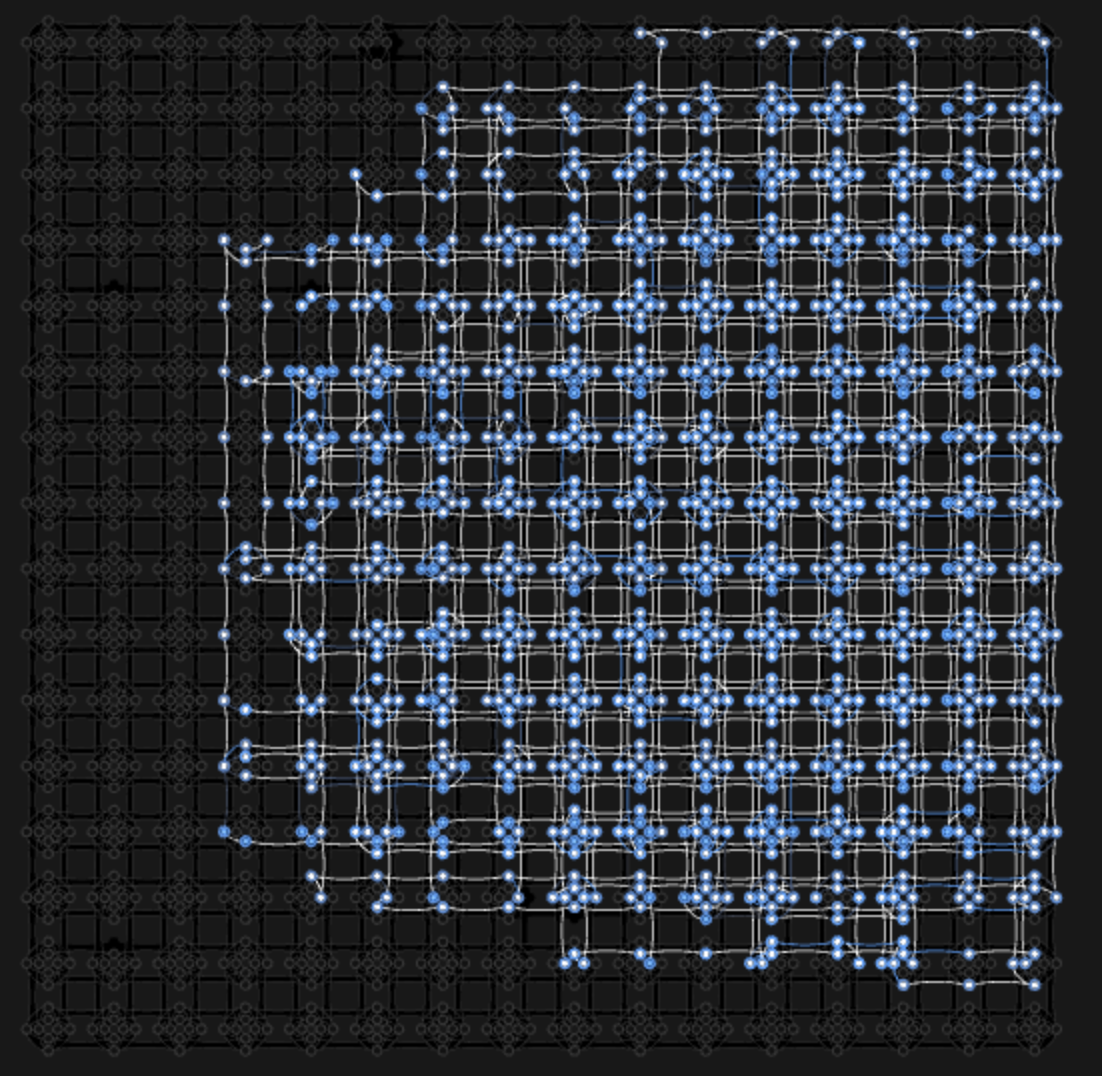
\includegraphics[width=0.3\textwidth]{chimera}
            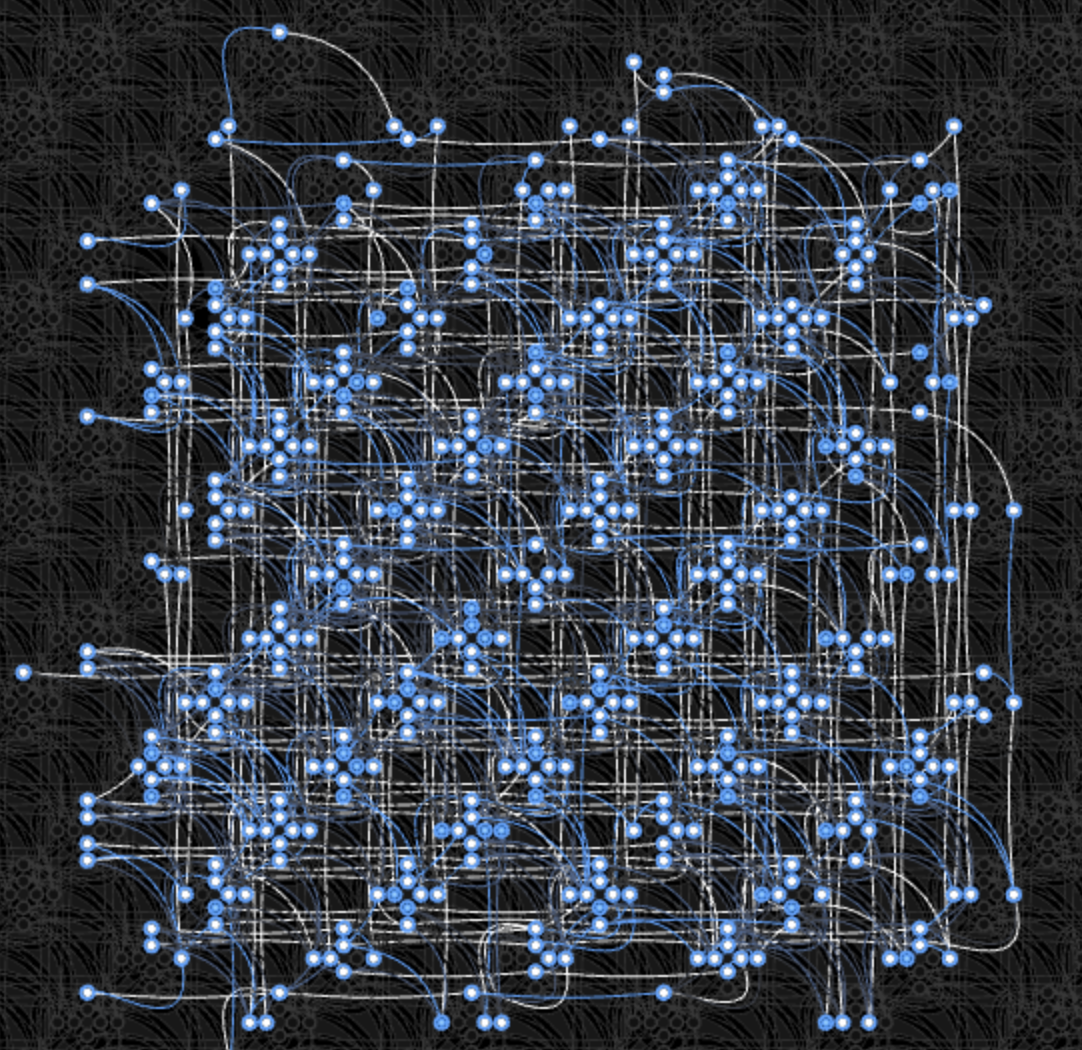
\includegraphics[width=0.3\textwidth]{pegasus}
            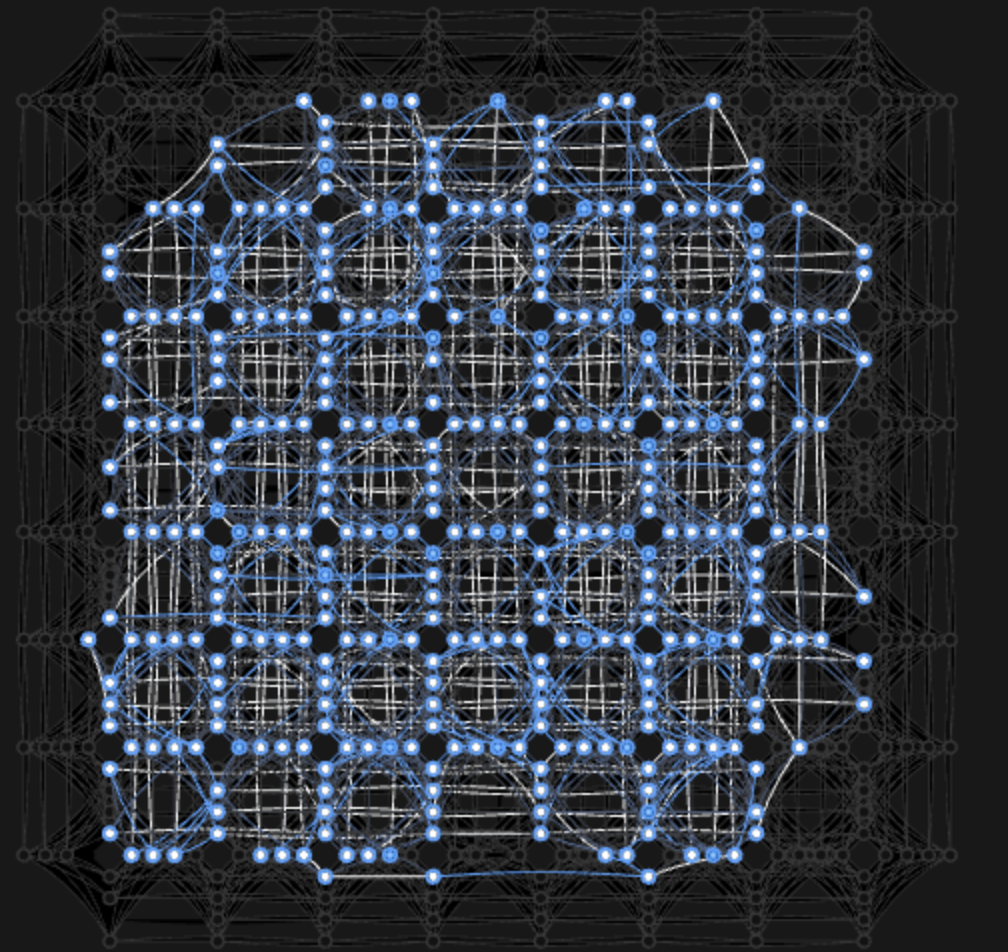
\includegraphics[width=0.3\textwidth]{zephyr}
            \caption{Mapping des différentes topologies avec dans l'ordre : Chimera, Pegasus, Zephyr}
            \label{fig:topologies_mapping}
        \end{figure}


        On observe que la dernière topologie, à savoir Zephyr, obtient de bien meilleur résultats, avec près de 10\% de solutions possibles trouvées, et une moyenne d'energie plus basse, et donc de meilleures chemins.
        Cependant cette topologie est encore très limité par son nombre de qbits, et on peut donc s'attendre à plus de possibilités dans les années à venir.




        \subsection{Comparaison avec les algorithmes classiques}\label{subsec:comparaison-avec-les-algorithmes-classiques}

        Afin de comparer nos resultats avec les algorithmes classiques, nous avons utilisé le simulated annealing que nous avons codé en python.\\
        Le fonctionnement de cet algorithme est quelque peu similaire à celui de la machine D-Wave, puisqu'il utilise un recuit, c'est à dire une diminution de la température( contrairement à la machine D-Wave, qui diminue la solution initiale).\\
        Nous avons donc utilisé la même instance de 10 villes, et nous avons comparé les résultats obtenus avec les algorithmes classiques, et ceux obtenus avec la machine D-Wave.\\
        Les paramètres utilisés sont les suivants : \\
        \begin{itemize}
            \item Annealing time : 100
            \item Num reads : 2500
            \item Lambda : 75
            \item Topology : Pegasus
        \end{itemize}
        On obtient les résultats suivants :\\
        \begin{table}[h]
            \centering
            \begin{tabular}{|c|c|c|}
                \hline
                \textbf{Algorithme} & Simulated Annealing & D-Wave  \\ \hline
                \textbf{Tps d'execution} & 1.62s & 64.5s  \\ \hline
                \textbf{Meilleure solution} & 294 & 347 \\ \hline
            \end{tabular}
            \caption{Résultats pour les différentes topologies}
            \label{tab:algo_results}
        \end{table}\\
        \begin{figure}[h]
            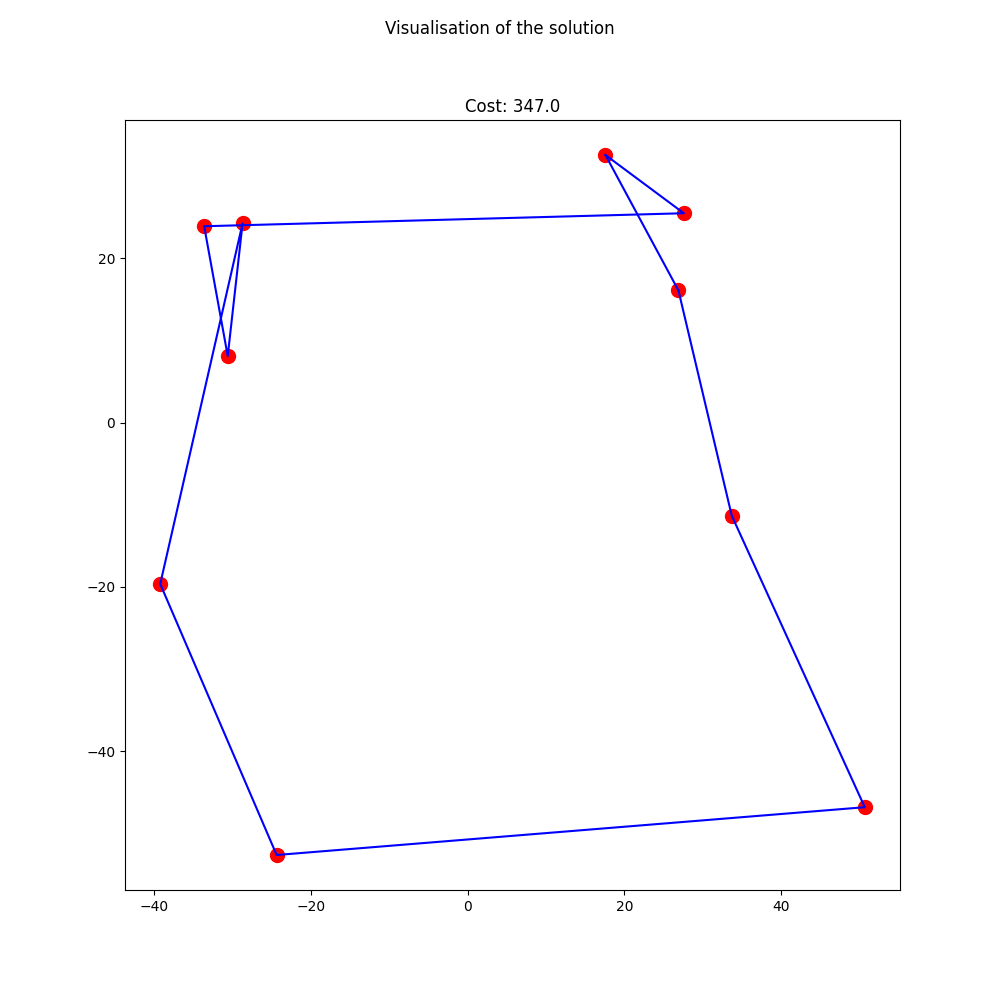
\includegraphics[width=0.5\textwidth]{quantum_annealing}
            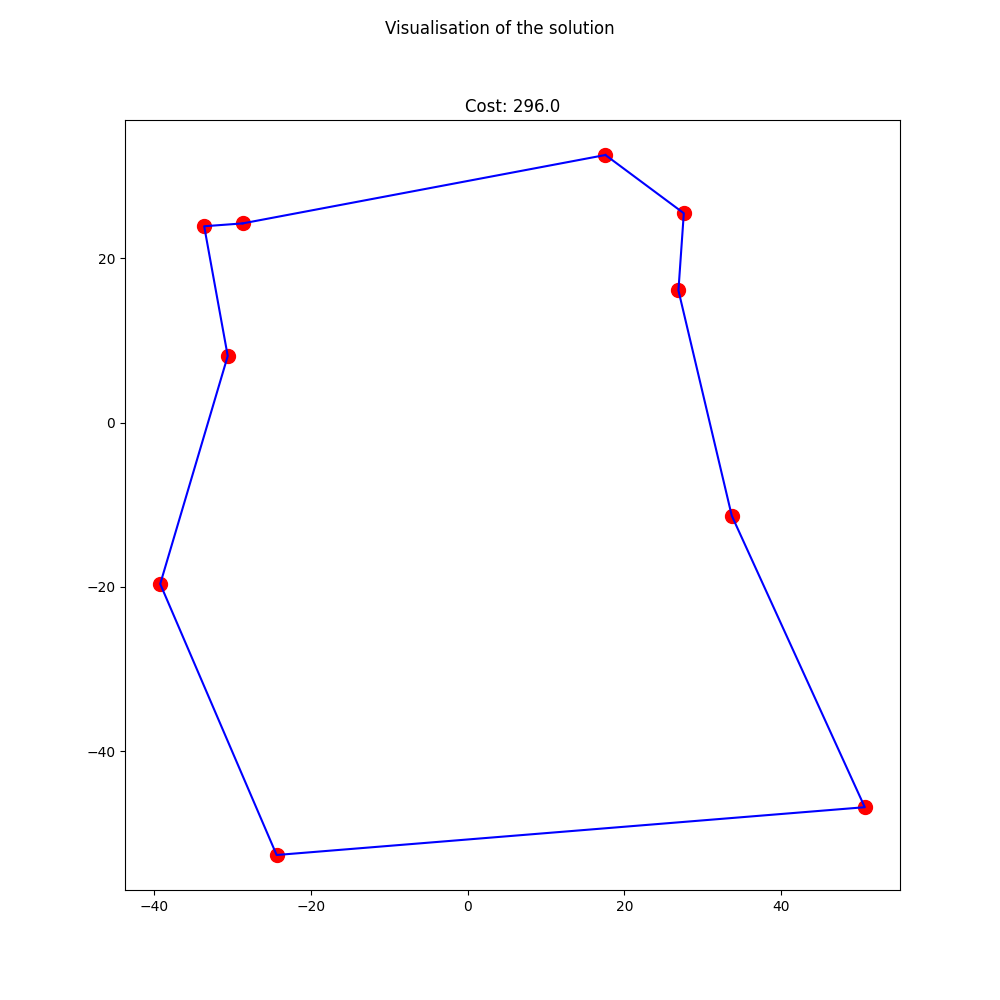
\includegraphics[width=0.5\textwidth]{simulated_annealing}
            \caption{Comparaison des algorithmes classiques et de la machine D-Wave\\
            à gauche : machine D-Wave, à droite : simulated annealings}
            \label{fig:comparaison}
        \end{figure}\\\\
        On constate que le simulated annealing est beaucoup plus rapide que la machine D-Wave, et que la solution trouvée est meilleure.\\
        La différence de temps d'execution n'est pas du à l'utilisation de la machine D-Wave, mais bien à l'utilisation de la topologie Pegasus, mais à l'embeding des qbits.\\
        En effet, l'embedding (ou mapping) est le processus qui permet de convertir les contraintes du problème à résoudre en contraintes de couplage entre les qbits.\\
        Cependant, l'embedding est un processus très complexe, et qui peut prendre beaucoup de temps. Comme c'est un problème d'optimisation en lui même, et donc entraine un temps de calcul important.\\
        La différence de coût quand à elle, est due au fait que les qbits ne sont pas tous connectés entre eux, et donc il faut passer par des qbits intermédiaires.\\
        Cela crée du bruit, et donc augmente le coût de la solution.\\





        \section{Generalized Travelling salesman problem}

        Le GTSP est une extension du TSP classique dans laquelle les villes sont regroupées en ensembles appelés clusters. Le but est de trouver le chemin le plus court qui passe par au moins une ville de chaque cluster. Cela signifie que le voyageur de commerce n'a pas besoin de visiter toutes les villes, mais doit en visiter au moins une de chaque cluster. Le GTSP est donc plus flexible que le TSP classique car il permet au voyageur de commerce de sauter certaines villes tout en visitant toutes les régions.\\\\
        Le GTSP peut être considéré comme un problème de tournée de véhicules avec des contraintes supplémentaires. Dans ce problème, le voyageur de commerce doit parcourir les clusters dans un ordre spécifique tout en minimisant la distance totale parcourue.\\\\
        Soit C l'ensemble des clusters, on obtient alors comme QUBO:

        \begin{equation*}
            \sum_{p=1}^{|C|} \sum_{k=1}^{|C|}\sum_{i \in C_k}\sum_{\substack{j=1 \\ j \notin C_k}}^{|X|}d_{ij}x_{ip}x_{j(p+1)} + \lambda\sum_{p=1}^{|C|}\sum_{k=1}^{|C|}(\sum_{i \in C_k}x_{ip}-1)^2 + \lambda\sum_{k=1}^{|C|}\sum_{i \in C_k}(\sum_{p=1}^{|C|}x_{ip} - 1)^2
        \end{equation*}


        Lorsque le nombre de clusters est égal au nombre de villes, le GTSP devient le TSP classique.\\\\
        Comme résultat, on obtient un chemin qui passe par au moins une ville de chaque cluster, et qui minimise la distance totale parcourue.
        En comparaison avec le TSP, nous pouvons avoir une instance de GTSP avec un nombre de villes plus grand.
        En effet, il y a moins de contraintes, et donc moins de connections entre les qbits.\\\\


        \section{Conclusion}

        Nous avons pu voir que la machine D-Wave permet de résoudre des problèmes NP-complets comme le TSP, et le GTSP.\\
        Cette machine est donc très prometteuse, et permettra de résoudre des problèmes plus complexes dans les années à venir.\\
        Cependant, il reste encore beaucoup de travail à faire, et notamment sur l'embedding, qui est un processus très complexe, et qui peut prendre beaucoup de temps.\\
        En effet, l'embedding est un problème d'optimisation en lui même, et donc entraine un temps de calcul important.
        Cela augmente donc grandement le temps d'execution, et donc le coût de la solution.\\
        De même, la limite de connectivité des qbits restreint la qualité des solutions trouvées, puisqu'il faut passer par des qbits intermédiaires.\\





    \end{document}
